\documentclass[numbers=endperiod]{scrartcl}
%%% Font packages
\usepackage{tgpagella}\setkomafont{disposition}{\rmfamily\bfseries}
\usepackage[T1]{fontenc}
\usepackage[utf8]{inputenc}
%%%
\usepackage{tikz}
%%% Taal & bettere typografie packages
\usepackage[dutch]{babel}
\usepackage[activate={true,nocompatibility},final,tracking=true,kerning=true,spacing=true,factor=1100,stretch=10,shrink=10]{microtype}
\microtypecontext{spacing=nonfrench}
%%% Wiskunde & fysica
\usepackage{amsmath,amssymb,amsthm}
\numberwithin{equation}{section}

%%%%Herdefiniëring van de wortel-teken
\usepackage{letltxmacro}
\makeatletter
\let\oldr@@t\r@@t
\def\r@@t#1#2{%
    \setbox0=\hbox{$\oldr@@t#1{#2\,}$}\dimen0=\ht0
    \advance\dimen0-0.2\ht0
    \setbox2=\hbox{\vrule height\ht0 depth -\dimen0}%
{\box0\lower0.4pt\box2}}
\LetLtxMacro{\oldsqrt}{\sqrt}
\renewcommand*{\sqrt}[2][\ ]{\oldsqrt[#1]{#2} }
\makeatother

\usepackage{siunitx}
\sisetup{output-decimal-marker = {,}}
%%%
\usepackage{graphicx}
\usepackage{multirow,booktabs}
%%% Verwijzingen & hyperlinks
\usepackage{hyperref}
\usepackage[dutch]{cleveref}
%%%%
\KOMAoptions{DIV=calc,BCOR=.75cm, abstract=true}


\renewcommand*\descriptionlabel[1]{\hspace\labelsep
  \normalfont\bfseries\MakeUppercase{#1}}% Make description environment label bold
\setlength{\parindent}{0pt}
%%% Front matter
\begin{document}
%Effe een titel gemaakt met geschikte logo...
\begin{titlepage} 
	\newcommand{\HRule}{\rule{\linewidth}{0.5mm}} % \Hrule is gelijk aan een een horizontale lijn met de lengte van een tekstlijn en dikte van een halve milimeter
	
	\center % Centralisatie van de elementen die volgen na deze command
	
	%------------------------------------------------
	%	Titels/subtitels
	%------------------------------------------------
	
	\textsc{\LARGE Lyceum}\\[1.5cm] % Onze school
	
	\textsc{\Large Kinematica}\\[0.5cm] % Hoofdonderwerp 
	
	\textsc{\large Fysica}\\[0.5cm] % Het vak
	
	%------------------------------------------------
	%	Titel
	%------------------------------------------------
	
	\HRule\\[0.4cm] %\\[<lengte>] is afstand tussen de hoofdtitel en lijn(Hrule)
	
	{\huge\bfseries Invloed luchtweerstand op valversnelling}\\[0.4cm] % Hoofdtitel
	
	\HRule\\[1.5cm]
	
	%------------------------------------------------
	%	Schrijvers
	%------------------------------------------------
	
	\begin{minipage}{0.4\textwidth}
		\begin{flushleft} %De tekst begint links
			\large
			\textit{Auteur}\\
			Fidon \textsc{Namani}\\ % Ik
		
		\end{flushleft}
	\end{minipage}
	~ % Dit golfje geeft aan dat deze twee minipagina's nooit onder elkaar mogen komen te staan.
	\begin{minipage}{0.4\textwidth}
		\begin{flushright} %De tekst begint rechts
			\large
			\textit{Beoordelaar}\\
			 \textsc{E. Zijlstra} % Beoordelaar
		\end{flushright}
	\end{minipage}


	
	%------------------------------------------------
	%	Datum
	%------------------------------------------------
	
	\vfill\vfill\vfill % De datumverschijning is 3/4 lengte van top van papier geplaatst.
	
	{\large\today} % Datum
	
	%------------------------------------------------
	%	Logo
	%------------------------------------------------
	
	\vfill\vfill
%	\includegraphics[width=0.7\textwidth]{seesaw}\\[1cm] % Ons fysica logootje
	 
	%----------------------------------------------------------------------------------------
	
	\vfill %De datum wordt voor de zekerheid nog 1/4 deel van de bodem van papier naar boven geduwd
\end{titlepage}
%%

\hrule
\begin{abstract}
    \textit{Doel}: Het doel van dit experiment was om een experiment uit te voeren en de resultaten van het model te vergelijken met de resultaten van het eerste model. Hieruit kan worden geconcludeerd of de uitgangspunten van het model realistisch waren.
    
    Bij dit proefje wordt experimenteel onderzocht hoe het waterpeil in een cilinder verandert in de loop van de tijd. Van de wijzigingen van het waterpeil worden diagrammen gemaakt.  

    \textit{Methode}:

    \textit{Resultaten \& Discussie}:

    \textit{Conclusie}:
\end{abstract}
\hrule
\newpage
\section{Inleiding}
Vaak wordt op het nieuws uitgezonden over olielekkage van grote vrachtschepen. De olie zal over een grote oppervlakte op het water gaan uitstromen. De uitstroom van de olielekkage hangt af van een aantal bepaalde factoren. Zal de uitstroom toenemen naarmate de lekkage groter wordt? Neemt de uitstroom af als het volume in de tank vermindert? Beantwoording vereist een analyse van de vloeistofdynamica van een olielekkage. Deze analyse is ook afleidbaar door de vloeistofdynamica van een leeglopende cilinder te onderzoeken. In deze proef werd de vloefstofdynamica van een leeglopende emmer geanalyseerd met behulp van \textit{Coach7} en modellering. De beantwoording van de volgende vragen was beoogd:

\begin{description}
\item[Hoofdvraag:] Wat is het verband tussen volumeafname en tijd bij het leeglopen van emmer?

\item[Deelvraag 1:] Wat voor verband bestaat er tussen de hoogte van het water en de tijd?

\item[Deelvraag 2:] Hoe hangt de stroomsnelheid af van het vloeistofpeil in het object?

\item[Deelvraag 3:] Wat voor verband bestaat er tussen de hoogte van het water en de instroom?

\item[Deelvraag 4:] Wat is het verband tussen de constante instroom en uitstroom?
\end{description}

\newpage
\section{Theorie}
De uistroomsnelheid hangt af van de hoogte en de tijdsconstante. De wet van Torricelli kan hier worden toegepast en daarbij geldt de wet van behoud van energie. Hoogte-energie wordt namelijk omgezet in snelheid. De volgende vergelijking kan hierbij worden opgesteld:
\begin{align}
    \begin{split}
        m \cdot g \cdot h_i = \frac{1}{2} \cdot m \cdot v^2 \Rightarrow
        \vec{v} = \sqrt{2 \cdot g \cdot h_i}
    \end{split}
\end{align}
Hierbij hangt $v$ niet liniear samen af met de hoogte

Op basis van de bovengenoemde theorie waren de volgende hypotheses opgesteld:
\begin{itemize}
 \renewcommand{\labelitemi}{\scriptsize$\blacksquare$}
    \item Een wortelverband bestaat tussen $y$ en $t$.
    \item Een liniear verband bestaat tussen $v(h)$ en $t$.
\end{itemize}

\newpage
\section{Methode}
Bij het experiment is gebruik gemaakt van een rolmaat en een object die cilindervormig is, voor de inhoud van een cilinder geldt de \ref{eq:cilinder}. 
\begin{equation}\label{eq:cilinder}
    I_{cilinder} = \pi \cdot r^2 \cdot h
\end{equation}
Voor het uitstromen van de cilinder is er perforatie toegepast. Eén individu  reguleerde het openen en sluiten van de opening. Een ander individu ging met een stopwatch op een gelijke tijdsinterval van \SI{10}{\second} bijhouden en meet de hoogte van het water met een rolmaat met een $\pm$ \SI{1}{\milli\meter} precisie. De resultaten zijn ingevoerd in \textit{Coach 7}. Met behulp van de modelleringscapaciteiten van \textit{Coach 7} was een $h$ als van functie van $t$ grafiek gemaakt.  






%Bij het experiment is gebruik gemaakt van een rolmaat en een blik. De stralen van de cirkels werden gemeten met een rolmaat met een \SI{1}{\centi\meter}. Voor de de uitkomst van de oppervlakte het blikje geld de volgende vergelijking:
\begin{equation}
    A_1 = \pi \cdot 0.098^2 = \SI{3.017e-2}{\meter\squared}
\end{equation}
 De formule voor de oppervlakte van de opening is soortgelijk.
\begin{equation}
    A_2 = \pi \cdot 0.002^2 = \SI{1.2566e-5}{\meter\squared}
\end{equation}

%Eén individu hield de smalle blik vast en was in bediening van het openen en sluiten van opening. Het andere individu ging met een smartphone de tijd meten. Op gelijke tijdsintervallen van \SI{10}{\second} werd de opening gauw gesloten en vervolgens werd met een rolmaat de momentele hoogte gemeten. De resulterende gegevens werden ingevoerd in \textit{Coach 7} opgenomen. Met behulp van %modelleren van \textit{Coach 7} waren de overige grootheden bepaald op $x$
\begin{figure}[ht]
\centering
\caption{Een schematische weergave van de opstelling.}
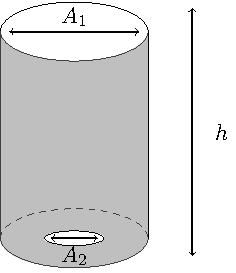
\includegraphics[scale=0.8]{Beker.pdf}    
\end{figure}

\newpage
\section{Formules}
De hoeveelheid volume van een vloeistof dat per tijdseenheid door een zekere oppervlakte passeert, wordt het debiet genoemd. Mathematisch omschreven als volgt:
\begin{equation}\label{eq:debiet}
    Q = \frac{dV}{dt}.
\end{equation}
Volume is oppervlakte waardoor het vloeistof maal de hoogte van dit vloeistof. Hieruit volgt dat $Q$ equivalent is aan het volgende:
\begin{equation}\label{eq:debiet_omschreven}
    Q = \frac{dV}{dt} = \frac{dhA}{dt} = A\frac{dh}{dt} = Av.
\end{equation}
In \cref{eq:debiet_omschreven} is $v$ de snelheid van vloeistof in \si{\meter\per\second} door oppervlakte $A$.

Op elke plek in het gevulde gedeelte van het vat is het debiet gelijk. 
\begin{equation}\label{eq:constant_debiet}
    Av = \text{constant}
\end{equation}

Het doorsnee oppervlakte verschilt weliswaar. Zo is bij het gat $A_1 < A_2$. Uit \cref{eq:constant_debiet} volgt dan:
\begin{equation}
\begin{split}
    A_1\vec{v}_1 = A_2\vec{v}_2\\
    \vec{v}_2 = \frac{A_1}{A_2}\vec{v}_1\\
     \rightarrow v_2 = -\frac{A_1}{A_2}v_1\\
    \end{split}
    \end{equation}
% Eenheden van een grootheid wordt weergeven als volgt: [grootheid]
$[v_{\text{stroom}}]$ is gelijk aan \si{\meter\per\second}. Uit \cref{eq:eenheid} volgt dat $c$ gelijk is aan:
\begin{equation}\label{eq:eenheid}
[c] = \frac{[v_{(\text{stroom})}]}{[h]} = \frac{\si{\meter\per\second}}{\si{\meter}} = \si{\second}^{-1}
\end{equation}
De constante $c$ heeft dus als eenheid $\si{\second}^{-1}$


%\section{Methode}

%\begin{figure}
%    \centering
%    \includegraphics[scale=0.4\textwidth]{main tex(1)}
%    \caption{Een schematische weergave van de opstelling.}
%    \label{fig:nigger}
%\end{figure}

\newpage
\section{Extra opdrachten}
\begin{table}[ht]
 \caption{Een schematische overzicht van alle data van model 1.}
    \label{tab:1}
    \centering
    \begin{tabular}{c c c} 
    \toprule
      h(\si{\milli\meter})&t(\si{\second})\\
    \midrule
   \num{3.0e+2} & 0.00 \\ 
   \num{2.3e+2} & 10.00\\
   \num{1.8e+2} & 20.00\\ 
   \num{1.4e+2} & 30.00\\ 
   \num{1.1e+2} & 40.00\\ 
    86 & 50.00\\ 
    67 & 60.00\\ 
    52 & 70.00\\
    40 & 80.00\\
    32 & 90.00\\
    25 & 100.00\\
    19 & 110.00\\ 
    15 &120.00 \\
    \bottomrule
    \end{tabular}
\end{table}
Elk willekeurig punt uit \ref{tab:1} kan worden geselecteerd om vervolgens de constante, oftewel ($\lambda$) te berekenen:
\begin{equation}\label{eq:lambda}
h(t) =h(0) \cdot e^{-\lambda t}
\Rightarrow \lambda = -\frac{\ln\left(\frac{h(t)}{h(0)}\right)}{t}.
\end{equation}
Vergelijking \ref{eq:lambda} beschrijft een functie tussen de constante ($\lambda$) en de initiale hoogte $h_i$. In de proef kan met behulp van de verkregen data en algebraïsche omgeschreven vergelijking \ref{eq:lambda} de ($\lambda$) worden berekend. De constante, oftewel ($\lambda$) wordt weergeven in \ref{eq:lambda}:
\begin{equation}
\begin{split}
-\frac{\ln\left(\frac{h(t)}{h(0)}\right)}{t}=-\frac{\ln\left(\frac{0.233567}{0.30}\right)}{10.00}=-0.0250.  
\end{split}
\end{equation}
Het verkregen antwoord uit \ref{eq:lambda} wordt vergeleken met \textit{Coach 7}. Voor het vergelijken van het antwoord wordt ... geanalyseerd en vervolgens met de handeling functie-fit, wordt het functietype: $f(x)=a \cdot exp(bx)+c$ geselecteerd. De optie schatting wordt geselecteerd en vervolgens worden de variabelen $a$ en $c$ respectievelijk vastgezet op $a=0.30$ en $c=0$, tot slot wordt de optie verfijnd. De verkregen waarde van $b$ komt nauwkeurig overeen met de waarde van \ref{eq:lambda}, namelijk $\lambda=-0.0250$.

Bij exponentiële afname is de halveringstijd de tijd waarin de hoeveelheid wordt gehalveerd. Bij groeifactor $e$ kan de halveringstijd $t$ worden berekend door de vergelijking $e^{-\lambda t}$ op te lossen.
\begin{equation}
e^{-\lambda t} = \frac{1}{2} \Rightarrow t =\frac{\ln(\frac{1}{2})}{-0.0250} = \SI{27.691}{\second}.
\end{equation}



De halveringstijd, oftewel $t_{\frac{1}{2}}$, wordt weergeven in \ref{eq:half}.
\begin{equation}\label{eq:half}
 t_{\frac{1}{2}}=\frac{\frac{\log\left(\frac{h(t)}{h(0)}\right)}{\log(\frac{1}{2})}}{t}
\end{equation}
Voor een exponentiële functie geldt het volgende functietype: $f(x) = a \cdot exp(bx)+c$. De richtingscoëfficiënt kan worden bepaald door twee punten uit de grafiek te selecteren. $a=\frac{\Delta y}{\Delta x}$ oftewel, $a=\frac{\Delta h}{\Delta t}$.  

\begin{align}\label{eq:A}
\begin{split}
v(h) = -\frac{A1}{A2} \cdot c \cdot h \Rightarrow -\frac{A1}{A2} \cdot c =\frac{v(h)}{h(t)}\\
-\frac{A1}{A2} \cdot c = \frac{-0.0075}{0.3} = -0.0250
\end{split}
\end{align}
Het verkregen antwoord van \ref{eq:A} komt exact overeen met de $\lambda$ uit de functie $h(t) = h(0)\cdot e^{\lambda t}$.

\newpage
\section{Bonus}
Aangenomen geldt dat $-\lambda = -\frac{A_1}{A_2} \cdot c$. Hieruit volgt dat $v(h) = \lambda \cdot h(0)$

\begin{equation}
-\lambda = -\frac{A_1}{A_2} \cdot c    
\end{equation}
Hieruit volgt dat $v(h)$ equivalent is aan het volgende:
\begin{equation}
v_{(stroom)} = c \cdot h \Rightarrow v(h) = -\lambda \cdot h(0)
\end{equation}

\newpage
\section{Reflectie}
Ik ben tevreden met de resultaten van ons uitgevoerde onderzoek. Daarnaast
ben ik trots op ons verslag. De gegevens zijn op een professionele
manier in het verslag verwerkt met een mooie strakke lay-out. Ik ben minder
tevreden met de meetfouten die zijn gemaakt. Ondanks dat ik de theorie
goed hebben toegepast. Ik heb in deze PO geleerd om onze kennis in
een praktische opdracht toe te passen, waardoor ik de onderzoeksvragen
heb kunnen beantwoorden.


\newpage
\appendix
\section{Logboek}
\begin{table}[ht]
\centering
\caption{Een logboek met de van week van uitvoering, activiteit, tijdspendering.}
\begin{tabular}{Scc}
\toprule
{Week van uitvoering} & Activiteit & Tijdspendering in (\si{\hour})\\
\midrule
6 & Oriënteren & 1\\
7 & Oriënteren & 1\\
8 & Oriënteren & 1\\
9 & videometing & 2\\
10 & Dataverwerking & 2\\
11 & Dataverwerking & 2\\
12 & Afronding & 1\\
13 & Controle & $\frac{1}{6}$\\
\bottomrule
\end{tabular}
\end{table}
\end{document}
